\documentclass{article}

\usepackage{amsmath,amssymb}
\usepackage{tikz}
\usepackage{pgfplots}
\usepackage{xcolor}
\usepackage[left=2.1cm,right=3.1cm,bottom=3cm,footskip=0.75cm,headsep=0.5cm]{geometry}
\usepackage{enumerate}
\usepackage{enumitem}
\usepackage{marvosym}
\usepackage{tabularx}
\usepackage{hyperref}
\usepackage{longtable}

\usepackage{listings}
\definecolor{lightlightgray}{rgb}{0.95,0.95,0.95}
\definecolor{lila}{rgb}{0.8,0,0.8}
\definecolor{mygray}{rgb}{0.5,0.5,0.5}
\definecolor{mygreen}{rgb}{0,0.8,0.26}
\lstdefinestyle{java} {language=java}
\lstset{language=java,
	basicstyle=\ttfamily,
	keywordstyle=\color{lila},
	commentstyle=\color{lightgray},
	stringstyle=\color{mygreen}\ttfamily,
	backgroundcolor=\color{white},
	showstringspaces=false,
	numbers=left,
	numbersep=10pt,
	numberstyle=\color{mygray}\ttfamily,
	identifierstyle=\color{blue},
	xleftmargin=.1\textwidth, 
	%xrightmargin=.1\textwidth,
	escapechar=§,
}

\usepackage[utf8]{inputenc}

\renewcommand*{\arraystretch}{1.4}

\newcolumntype{L}[1]{>{\raggedright\arraybackslash}p{#1}}
\newcolumntype{R}[1]{>{\raggedleft\arraybackslash}p{#1}}
\newcolumntype{C}[1]{>{\centering\let\newline\\\arraybackslash\hspace{0pt}}m{#1}}

\newcommand{\E}{\mathbb{E}}
\DeclareMathOperator{\rk}{rk}
\DeclareMathOperator{\Var}{Var}
\DeclareMathOperator{\Cov}{Cov}

\title{\textbf{Rechnernetze, Übung 10}}
\author{\textsc{Henry Haustein}}
\date{}

\begin{document}
	\maketitle
	
	\section*{Aufgabe 1}
	\begin{enumerate}[label=(\alph*)]
		\item Für jedes Pixel gibt es 256 $=2^8$ Werte, man braucht also 8 Bit = 1 Byte für die Speicherung. Inklusive Header braucht das Bild nun 54 Byte + $16^2\cdot 1$ Byte = 310 Byte.
		\item \underline{255 100 045} $\to$ Zeile 1-3 weiß + 1. Zeichen Zeile 4 = 49 Zeichen $\to$ 49-S = 45 \\
		\underline{000 100 000} $\to$ R Zeile 4 (4x schwarz) \\
		\underline{255 100 000} $\to$ Zwischenraum Zeile 4 (4x weiß) \\
		000 000 255 255 255 000 255 $\to$ Rest Zeile 4 $\to$ Summe Zeilen 1-4: 16 Byte \\
		255 000 255 255 255 000 255 255 255 000 255 000 255 255 000 255 $\to$ Zeile 5 (16 B) \\
		255 000 255 255 255 000 255 255 255 000 255 000 255 255 000 255 $\to$ Zeile 6 (16 B) \\
		255 000 255 255 255 000 255 255 255 000 255 255 000 255 000 255 $\to$ Zeile 7 (16 B) \\
		255 \underline{000 100 000} \underline{255 100 000} 000 255 255 000 255 000 255 $\to$ Zeile 8 (14 B) \\
		255 000 255 000 \underline{255 100 001} 000 255 255 000 255 000 255 $\to$ Zeile 9 (14 B) \\
		255 000 255 255 000 \underline{255 100 000} 000 255 255 000 255 000 255 $\to$ Zeile 10 (15 B) \\
		255 000 255 255 255 000 255 255 255 000 255 255 255 000 000 255 $\to$ Zeile 11 (16 B) \\
		255 000 255 255 255 000 255 255 255 000 255 255 255 000 000 255 $\to$ Zeile 12 (16 B) \\
		255 000 \underline{255 100 000} 000 255 255 000 \underline{255 100 000} 000 $\to$ Zeile 13 o. letztes Z. (13 B) \\
		\underline{255 100 045} $\to$ letztes Zeichen Zeile 13 + Zeilen 14-16 (3 B)
		\item Die 255 kommt am häufigsten vor, sie wird mit 1 Bit kodiert. Die 0 kommt am zweitöftesten vor, sie wird mit 2 Bit kodiert. 10 kommt am drittöftesten vor, sie wird mit 3 Bit kodiert.. 45 und 1 kommen am seltensten vor, sie werden mit 4 Bit kodiert. Insgesamt werden also $= 88 \cdot 1 \text{Bit} + 54 \cdot 2 \text{Bit} + 10 \cdot 3 \text{Bit} + 2 \cdot 4 \text{Bit} + 1 \cdot 4 \text{Bit}= 238 \text{Bit}$ benötigt.
	\end{enumerate}

	\section*{Aufgabe 2}
	\begin{enumerate}[label=(\alph*)]
		\item Tabelle
		\begin{center}
			\begin{tabular}{c|C{5cm}|C{5cm}}
				& \textbf{Signalisierung (SIP mit Beschreibungsformat SDP)} & \textbf{Transport (RTP, RTCP)} \\
				\hline
				Aufgabe & Aufbau und Aushandlung von Sessions & effiziente Datenübertragung \\
				\hline
				Topologie & meist über SIP Proxy & meist direkte Übertragung oder über MCU (Multipoint Control Unit) \\
				\hline
				Codierung & einfache Text-basierte Nachrichten & binär codiert, Einsatz von Audio-/Video-Codecs \\
				\hline
				Transportprotokoll & TCP oder UDP & nur UDP
			\end{tabular}
		\end{center}
		\item Systembild
		\begin{center}
			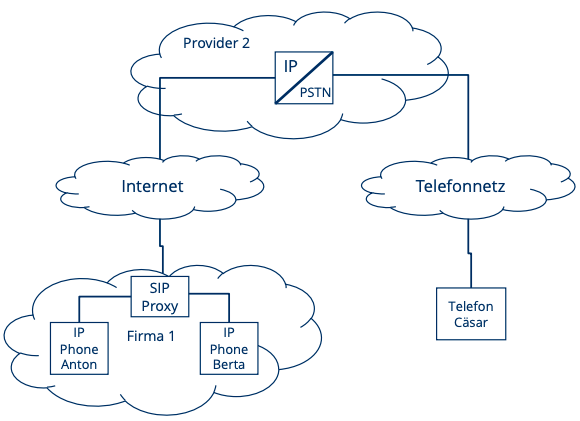
\includegraphics[width=0.75\textwidth]{./pics/Systembild}
		\end{center}
		\item Systembild mit Pfeilen
		\begin{center}
			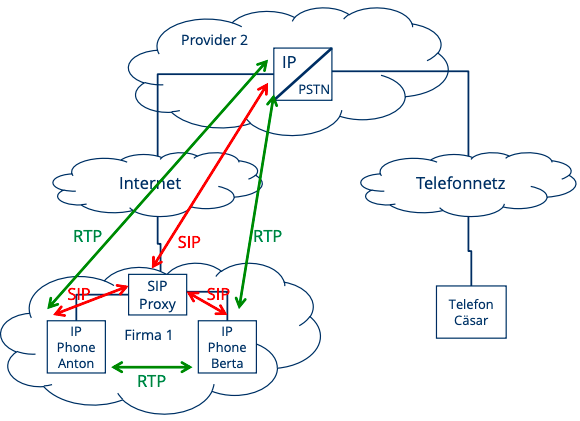
\includegraphics[width=0.75\textwidth]{./pics/Systembild_Pfeile}
		\end{center}
	\end{enumerate}

	\section*{Aufgabe 3}
	\begin{enumerate}[label=(\alph*)]
		\item Es gilt
		\begin{align}
			\text{Payload} &= \text{Datenrate} \cdot \text{Zeit} \notag \\
			&= 8\text{ kBit/s} \cdot 0.02\text{ s} \notag \\
			&= 160\text{ Bit} \notag
		\end{align}
		\item Durch den Overhead wächst die Größe eines Paketes auf 65 Byte. Bei 0.02 Sekunden pro Paket, also 50 Pakete pro Sekunde, ergibt sich eine Datenrate von $65\text{ Byte/Paket} \cdot 50\text{ Pakete/s} = 3250\text{ kByte/s}$.
	\end{enumerate}

	\section*{Aufgabe 4}
	\begin{enumerate}[label=(\alph*)]
		\item Ethernet II, IP, UDP
		\item Quelle: 200.57.7.204:8000, Ziel: 200.57.7.196:40376
		\item Version: RFC 1889 Version , Padding: 0, Extension: 0, Contributing source identifiers count: 0, Payload type: ITU-T G.711 PCMA, Sequence number: 3, Timestamp: 480
		\item Abtastfrequrnz von 8 kHz $\Rightarrow$ 0.125 ms pro Sample Abspielzeit $\Rightarrow$ 480. Sample startet bei $480\cdot 0.125\text{ ms} = 0.06\text{ s}$.
	\end{enumerate}

	\section*{Aufgabe 5}
	\begin{enumerate}[label=(\alph*)]
		\item Rohbandbreite:
		\begin{align}
			352\cdot 288\cdot 24\cdot 15 = 36.495.360 \text{ Bit/s} \approx 36.500\text{ kBit/s} \notag
		\end{align}
		Es stehen aber nur 192 kBit/s zur Verfügung, das heißt das Videosignal muss um den Faktor $\frac{36.500\cdot 1.2\text{ kBit/s}}{192\text{ kBit/s}}=228$ komprimiert werden.
		\item Jeder Teilnehmer sendet $\frac{36500\text{ kBit/s}}{250}=146\text{ kBit/s}$ an Daten. Mit Overhead sind das 175.2 kBit/s. Mit einem Downstream von 2048 kBit/s können also $\frac{2048\text{ kBit/s}}{175.2\text{ kBit/s}}\approx 11$ Teilnehmer senden.
	\end{enumerate}
	
\end{document}